\documentclass[usenames,dvipsnames,tikz]{standalone}
\usetikzlibrary{shapes.geometric}
\usepackage{xcolor}
\colorlet{tBlue}{RoyalBlue!35!Cerulean}
\colorlet{tRed}{Red}
\usepackage{tikz}
\usepackage{standalone}
\begin{document}
	
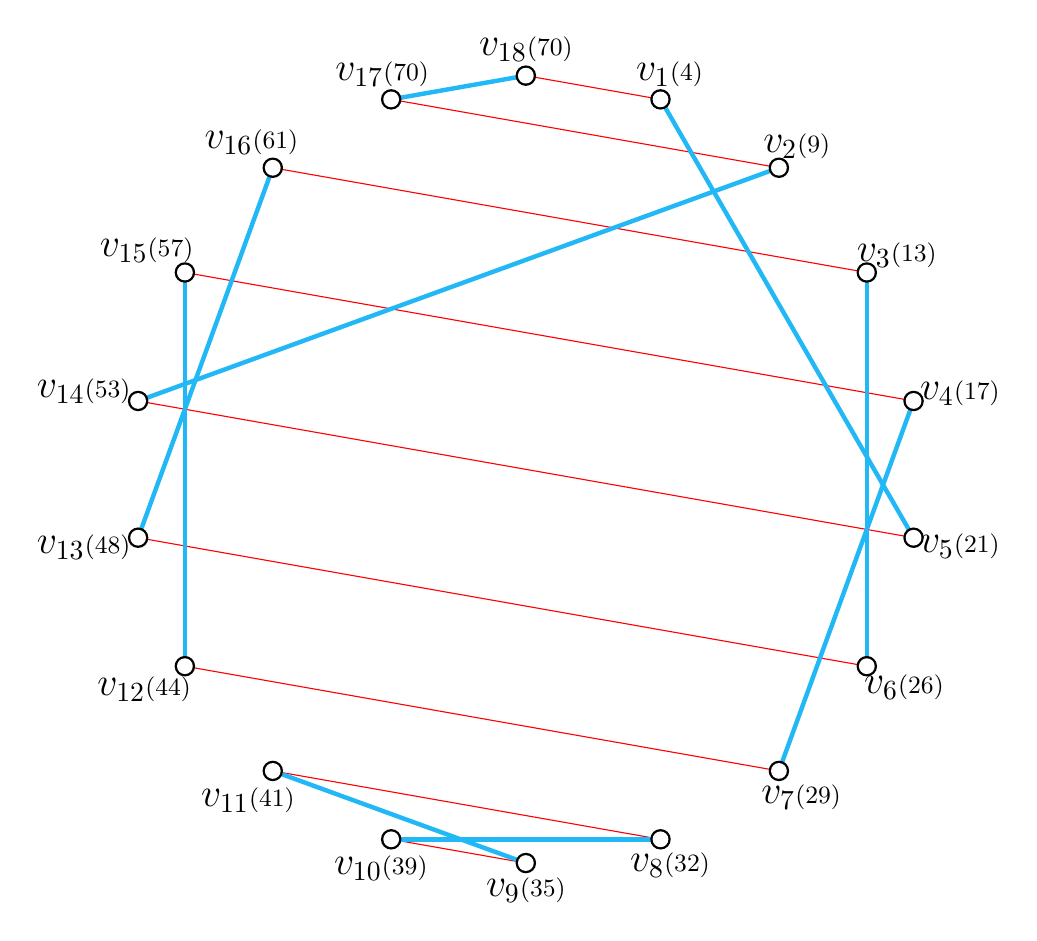
\begin{tikzpicture}
%Values of vertices:
% v1=4, v2=9, v3=13, v4=17, v5=21, v6=26, v7=29, v8=32, v9=35, v10=39, v11=41, v12=44, v13=48, v14=53, v15=57, v16=61, v17=70, v18=70 (v17/v18 universal vertices), \tau = 70.


\foreach \n/\value in {1/1, 2/1, 3/2, 4/2, 5/3, 6/4, 7/4, 8/5, 9/5, 10/6, 11/6, 12/6, 13/6, 14/7, 15/8, 16/9, 17/10, 18/10}
	\fill (90-\n*20:5cm) coordinate (v\n) circle [radius = 0.1];
	
\foreach \n/\value in {1/4, 17/70, 18/70}
	\fill (90-\n*20:5cm) coordinate (v\n) circle [radius = 0.1]
		++(90-\n*20:9.5pt) node {\Large{$v_{\n}$}\small{(\value)}};

\foreach \n/\value in {2/9, 8/32, 9/35}
	\fill (90-\n*20:5cm) coordinate (v\n) circle [radius = 0.1]
		++(90-\n*20:10pt) node {\Large{$v_{\n}$}\small{(\value)}};
		
\foreach \n/\value in {3/13, 7/29}
	\fill (90-\n*20:5cm) coordinate (v\n) circle [radius = 0.1]
		++(90-\n*20:12.5pt) node {\Large{$v_{\n}$}\small{(\value)}};		
		
\foreach \n/\value in {4/17, 5/21, 12/44}
	\fill (90-\n*20:5cm) coordinate (v\n) circle [radius = 0.1]
		++(90-\n*20:17pt) node {\Large{$v_{\n}$}\small{(\value)}};

\foreach \n/\value in {15/57}
	\fill (90-\n*20:5cm) coordinate (v\n) circle [radius = 0.1]
		++(90-\n*20:16pt) node {\Large{$v_{\n}$}\small{(\value)}};
	
\foreach \n/\value in {6/26}
	\fill (90-\n*20:5cm) coordinate (v\n) circle [radius = 0.1]
		++(90-\n*20:15.5pt) node {\Large{$v_{\n}$}\small{(\value)}};
		
\foreach \n/\value in {10/39}
	\fill (90-\n*20:5cm) coordinate (v\n) circle [radius = 0.1]
		++(90-\n*20:11pt) node {\Large{$v_{\n}$}\small{(\value)}};
		
\foreach \n/\value in {11/41}
	\fill (90-\n*20:5cm) coordinate (v\n) circle [radius = 0.1]
		++(90-\n*20:14pt) node {\Large{$v_{\n}$}\small{(\value)}};
		
\foreach \n/\value in {13/48, 14/53}
	\fill (90-\n*20:5cm) coordinate (v\n) circle [radius = 0.1]
		++(90-\n*20:20pt) node {\Large{$v_{\n}$}\small{(\value)}};	

\foreach \n/\value in {16/61}
	\fill (90-\n*20:5cm) coordinate (v\n) circle [radius = 0.1]
		++(90-\n*20:12pt) node {\Large{$v_{\n}$}\small{(\value)}};	
	
	
%Edges and vertices
\foreach \m/\n in {1/18, 2/17, 3/16, 4/15, 5/14, 6/13, 7/12, 8/11, 9/10}
	\draw [tRed] (v\n) -- (v\m);
\foreach \m/\n in {1/5, 2/14, 3/6, 4/7, 8/10, 9/11, 12/15, 13/16, 17/18}
	\draw [ultra thick, tBlue] (v\n) -- (v\m);
\foreach \n in {1,...,18}
	\fill (90-\n*20:5cm) coordinate (v\n) circle [radius = 0.13];
\foreach \n in {1,...,18}
	\fill [white] (90-\n*20:5cm) coordinate (v\n) circle [radius = 0.1];

\end{tikzpicture}
	
\end{document}